\section{Robustness against white noise}


The aim of this section is to study robustness against the addition of a white noise. 

Consider a Werner state 

\begin{equation}
    \rho = \beta \ket{\Phi}\bra{\Phi} + (1-\beta) \mathbbm{1}
\end{equation}

where $\ket{\Phi}$ is a maximally entangled state and $\mathbbm{1}$ a fully randomized behaviour. 


\begin{procedure}
\begin{enumerate}
    \item Start with $\beta = 1$ and a given precision $\delta$
    \item While the result of the primal is non local for the state $\rho$ : $\beta = \beta - \delta $
\end{enumerate}
\end{procedure}

Procedure 1 is applied by a dichotomic algorithm in order to have a good precision with the fewer iterations possible. 


% This file was created with tikzplotlib v0.10.1.
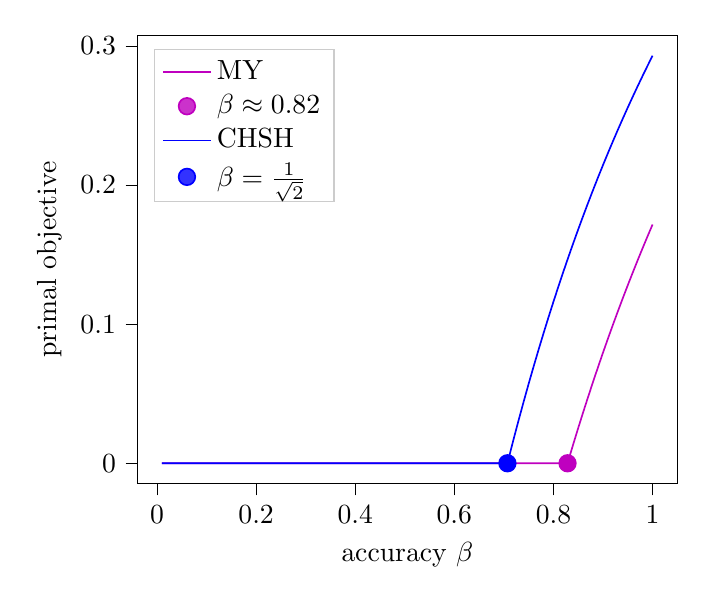
\begin{tikzpicture}

\definecolor{darkgray176}{RGB}{176,176,176}
\definecolor{darkviolet1910191}{RGB}{191,0,191}
\definecolor{lightgray204}{RGB}{204,204,204}

\begin{axis}[
legend cell align={left},
legend style={
  fill opacity=0.8,
  draw opacity=1,
  text opacity=1,
  at={(0.03,0.97)},
  anchor=north west,
  draw=lightgray204
},
tick align=outside,
tick pos=left,
x grid style={darkgray176},
xlabel={accuracy \(\displaystyle \beta\)},
xmin=-0.0395000000000008, xmax=1.0495,
xtick style={color=black},
y grid style={darkgray176},
ylabel={primal objective},
ymin=-0.0146446609406726, ymax=0.307537879754125,
ytick style={color=black}
]
\addplot [semithick, darkviolet1910191]
table {%
1 0.17157287525381
0.99 0.163204924498798
0.98 0.154666199238581
0.97 0.145951417787433
0.96 0.137055078389385
0.95 0.127971447635589
0.94 0.118694548142351
0.93 0.109218145434204
0.92 0.0995357339715324
0.91 0.0896405222569338
0.9 0.0795254169486775
0.89 0.069183005903157
0.88 0.0586055400611474
0.87 0.0477849140848387
0.86 0.0367126456439648
0.85 0.0253798532397762
0.84 0.0137772324450116
0.83 0.00189503042627678
0.82 0
0.81 0
0.8 0
0.79 0
0.78 0
0.77 0
0.76 0
0.75 0
0.74 0
0.73 0
0.72 0
0.71 0
0.7 0
0.69 0
0.68 0
0.67 0
0.66 0
0.65 0
0.64 0
0.63 0
0.62 0
0.61 0
0.6 0
0.59 0
0.58 0
0.57 0
0.56 0
0.55 0
0.54 0
0.53 0
0.52 0
0.51 0
0.5 0
0.49 0
0.48 0
0.47 0
0.46 0
0.45 0
0.44 0
0.429999999999999 0
0.419999999999999 0
0.409999999999999 0
0.399999999999999 0
0.389999999999999 0
0.379999999999999 0
0.369999999999999 0
0.359999999999999 0
0.349999999999999 0
0.339999999999999 0
0.329999999999999 0
0.319999999999999 0
0.309999999999999 0
0.299999999999999 0
0.289999999999999 0
0.279999999999999 0
0.269999999999999 0
0.259999999999999 0
0.249999999999999 0
0.239999999999999 0
0.229999999999999 0
0.219999999999999 0
0.209999999999999 0
0.199999999999999 0
0.189999999999999 0
0.179999999999999 0
0.169999999999999 0
0.159999999999999 0
0.149999999999999 0
0.139999999999999 0
0.129999999999999 0
0.119999999999999 0
0.109999999999999 0
0.0999999999999992 0
0.0899999999999992 0
0.0799999999999993 0
0.0699999999999993 0
0.0599999999999993 0
0.0499999999999993 0
0.0399999999999993 0
0.0299999999999992 0
0.0199999999999992 0
0.00999999999999925 0
};
\addlegendentry{MY}
\addplot [semithick, darkviolet1910191, mark=*, mark size=3, mark options={solid}, only marks]
table {%
0.828428781600444 0
};
\addlegendentry{$\beta \approx 0.82$}
\addplot [semithick, blue]
table {%
1 0.292893218813452
0.99 0.285750726074194
0.98 0.278462468176992
0.97 0.271023936921085
0.96 0.263430436264013
0.95 0.255677072435213
0.94 0.247758743418566
0.93 0.2396701277564
0.92 0.231405672623318
0.91 0.222959581113684
0.9 0.214325798681614
0.89 0.2054979986668
0.88 0.196469566833469
0.87 0.187233584843049
0.86 0.177782812573782
0.85 0.168109669192297
0.84 0.158206212873158
0.83 0.148064119052352
0.82 0.137674657089576
0.81 0.127028665201793
0.8 0.116116523516815
0.79 0.104928125080319
0.78 0.093452844632631
0.77 0.0816795049525354
0.76 0.0695963405440161
0.75 0.0571909584179363
0.74 0.0444502956938543
0.73 0.0313605737170578
0.72 0.0179072483520168
0.71 0.00407495607528462
0.7 0
0.69 0
0.68 0
0.67 0
0.66 0
0.65 0
0.64 0
0.63 0
0.62 0
0.61 0
0.6 0
0.59 0
0.58 0
0.57 0
0.56 0
0.55 0
0.54 0
0.53 0
0.52 0
0.51 0
0.5 0
0.49 0
0.48 0
0.47 0
0.46 0
0.45 0
0.44 0
0.429999999999999 0
0.419999999999999 0
0.409999999999999 0
0.399999999999999 0
0.389999999999999 0
0.379999999999999 0
0.369999999999999 0
0.359999999999999 0
0.349999999999999 0
0.339999999999999 0
0.329999999999999 0
0.319999999999999 0
0.309999999999999 0
0.299999999999999 0
0.289999999999999 0
0.279999999999999 0
0.269999999999999 0
0.259999999999999 0
0.249999999999999 0
0.239999999999999 0
0.229999999999999 0
0.219999999999999 0
0.209999999999999 0
0.199999999999999 0
0.189999999999999 0
0.179999999999999 0
0.169999999999999 0
0.159999999999999 0
0.149999999999999 0
0.139999999999999 0
0.129999999999999 0
0.119999999999999 0
0.109999999999999 0
0.0999999999999992 0
0.0899999999999992 0
0.0799999999999993 0
0.0699999999999993 0
0.0599999999999993 0
0.0499999999999993 0
0.0399999999999993 0
0.0299999999999992 0
0.0199999999999992 0
0.00999999999999925 0
};
\addlegendentry{CHSH}
\addplot [semithick, blue, mark=*, mark size=3, mark options={solid}, only marks]
table {%
0.707108195400103 0
};
\addlegendentry{$\beta = \frac{1}{\sqrt{2}}$}
\end{axis}

\end{tikzpicture}

\vspace{1cm}

For the CHSH game, we obtained $\beta^*_{CHSH} = 1/\sqrt{2} $ and for Mayer-Yao's correlations, $\beta^*_{MY}= \approx 0.82$. In each case, one can noticed that $\beta^* = 1 - \alpha^*$ where $\alpha^*$ was the optimal objective obtained in Section .. The study of the robustness was already given by the primal detecting non-local behaviour since it was written using a convex combination of the behaviour and a fully randomized behaviour which is actually a white noise. However, if one wants to study another type of noise, this study would be necessary. 

A conclusion we can draw is that the maximally entangled state is more robust for CHSH correlations than for Mayer-Yao's correlations. 


